\chapter{Trabajos Previos}



\section{Aprendizaje supervisado en la detección de emociones}



La detección automática de las respuestas internas que las personas reflejan en el texto, ante cierto fenómenos, ha sido estudiada con mucho interés en los últimos años. Es así como en \cite{pang2002thumbs} se  establece la importancia de desarrollar, ante textos que reflejen opiniones subjetivas, sistemas capaces de identificar si dicha opinión es negativa o positiva. Para este propósito, se emplea el dominio de las reviews online de películas, que facilitan la tarea, al contar con una clasificación negativa o positiva por parte del usuario, construyendo algoritmos de aprendizaje supervisado que utiliza como features principalmente unigramas, que es un elemento individual del texto y como variable objetivo la clasificación asignada. Por otro lado,  \cite{turney2002thumbs} pretende establecer a través de aprendizaje no supervisado, si determinada review sobre diversos temas online, presenta un sentimiento negativo o positivo. Para ello, emplea el concepto de orientación semántica presente en \cite{hatzivassiloglou1997predicting} para determinar si una frase tiene orientación negativa o positiva y así poder determinar si la review en su conjunto es positiva o negativa. En general, la determinación de la orientación negativa o positiva dentro del texto, es conocida como análisis de sentimiento

Así como en el análisis de sentimiento, contar con un corpus de términos que cuenten con una clasificación previa de su orientación, es clave para poder llevar a cabo automáticamente la tarea, para los estados emocionales  es igualmente importante, por lo que \cite{strapparava2004wordnet} realiza una anotación manual de estados emocionales basados en las categorías de \cite{ortony1987referential} sobre algunos términos encontrados en WordNet \cite{miller1995wordnet}, que es una base de datos de términos en ingles agrupados por grupos de sinónimos y con relación semántica entre grupos. A partir de las anotaciones manuales de las emociones de ciertos términos presentes en la base, se establece la categoría emocional de nuevos términos gracias a los sinónimos y las relaciones semánticas, construyendo así una base de datos de estados emocionales llamada WordNet-Affect. Dentro de esta misma linea, \cite{wiebe2005annotating}  elabora una anotación manual de las estados emocionales presentes en las oraciones de un gran volumen de noticias, en donde se tiene en cuenta el contexto. 

En el contexto de la clasificación automática de las emociones en el texto, \cite{alm2005emotions} utilizan los cuentos infantiles para desarrollar un modelo de aprendizaje supervisado capaz de detectar emociones en las frases. Para ello se elabora una anotación manual de las estas frases que constituyen el set de datos y luego, se generan un set de features para dichas frases que pasaran a entrenar un clasificador lineal.




\section{Redes neuronales para el análisis de texto}

Las técnicas tradicionales de análisis de emociones en el texto, están principalmente basadas en la relación que existe entre los términos que constituyen el texto y determinado estado emocional. Este tipo de análisis, si bien ha sido de gran utilidad, no dispone de la capacidad para tener en cuenta el contexto, es decir la relación que existe entre las palabras que constituyen el texto, ademas del orden en que estas se presentan. Debido a esto, recientemente el campo de estudio ha ido migrando hacia el uso del algoritmos capaces de captar esta relación contextual, específicamente las redes neuronales. 

Haciendo un recuento del estado del arte de la detección de emociones en el texto, \cite{acheampong2021transformer}  hablan de las distintas arquitecturas de redes neuronales usadas recientemente para esta tarea, entre ellas las RNN (redes neuronales recurrentes). Estas redes tienen un tipo de arquitectura cuyo uso es especial para datos secuenciales, tales como las tareas de NLP. En estas, para un ejemplo nuevo, es posible utilizar el resultado del procesamiento de un dato anterior, para el del siguiente dato (como en una secuencia de caracteres por ejemplo), es decir la misma topología de pesos recibirá para cada ejemplo nuevo, el resultado anterior ademas de la nueva entrada. Sin embargo, debido a su arquitectura, la optimizacion de los pesos que constituyen la topología de las RNN, se vuelve compleja para el calculo del gradiente del error, pues se deberá pasar tantas veces por los pesos de la red como pasos en el tiempo haya (como numero de caracteres en una palabra) haciendo que en secuencias particularmente largas, este calculo crezca en demasía.


Si bien las RNN permiten preservar de alguna manera la relación contextual del texto, al tener una estructura secuencial, se impide la paralelizacion de su computo, pues se necesita las salidas de ejemplos anteriores para llevar a cabo el siguiente paso en el tiempo. Ademas, debido a este mismo funcionamiento secuencial, si existe un gran numero de pasos en el tiempo, es poco probable que la red tenga en cuenta información presente al inicio. Para solucionar estos inconvenientes, \cite{vaswani2017attention} desarrollan los Transformers, que son un tipo de arquitectura en la que múltiples datos de entrada son ingresados a la red de manera simultanea, como todas las palabras en una frase por ejemplo. Esto se logra mediante la representación de dichas palabras en la forma de un vector y a través de una arquitectura que se define como atención. A partir de ahí, se realiza una transformación de los datos, de manera que la representación de cada dato, en este caso cada palabra, tenga en cuenta que tan importante es la misma para todas las demás palabras de la oración. Esta transformación, aplicada tanto en los datos de entrada como en los de salida, es luego usada para entrenar los pesos de la red. De esta manera la red es capaz de procesar datos en simultaneo así como tener en cuenta toda la información disponible. Un esquema de esta arquitectura se puede apreciar en la imagen \ref{figure:transformers} \cite{vaswani2017attention}.

\begin{figure}[t]
	\centering
	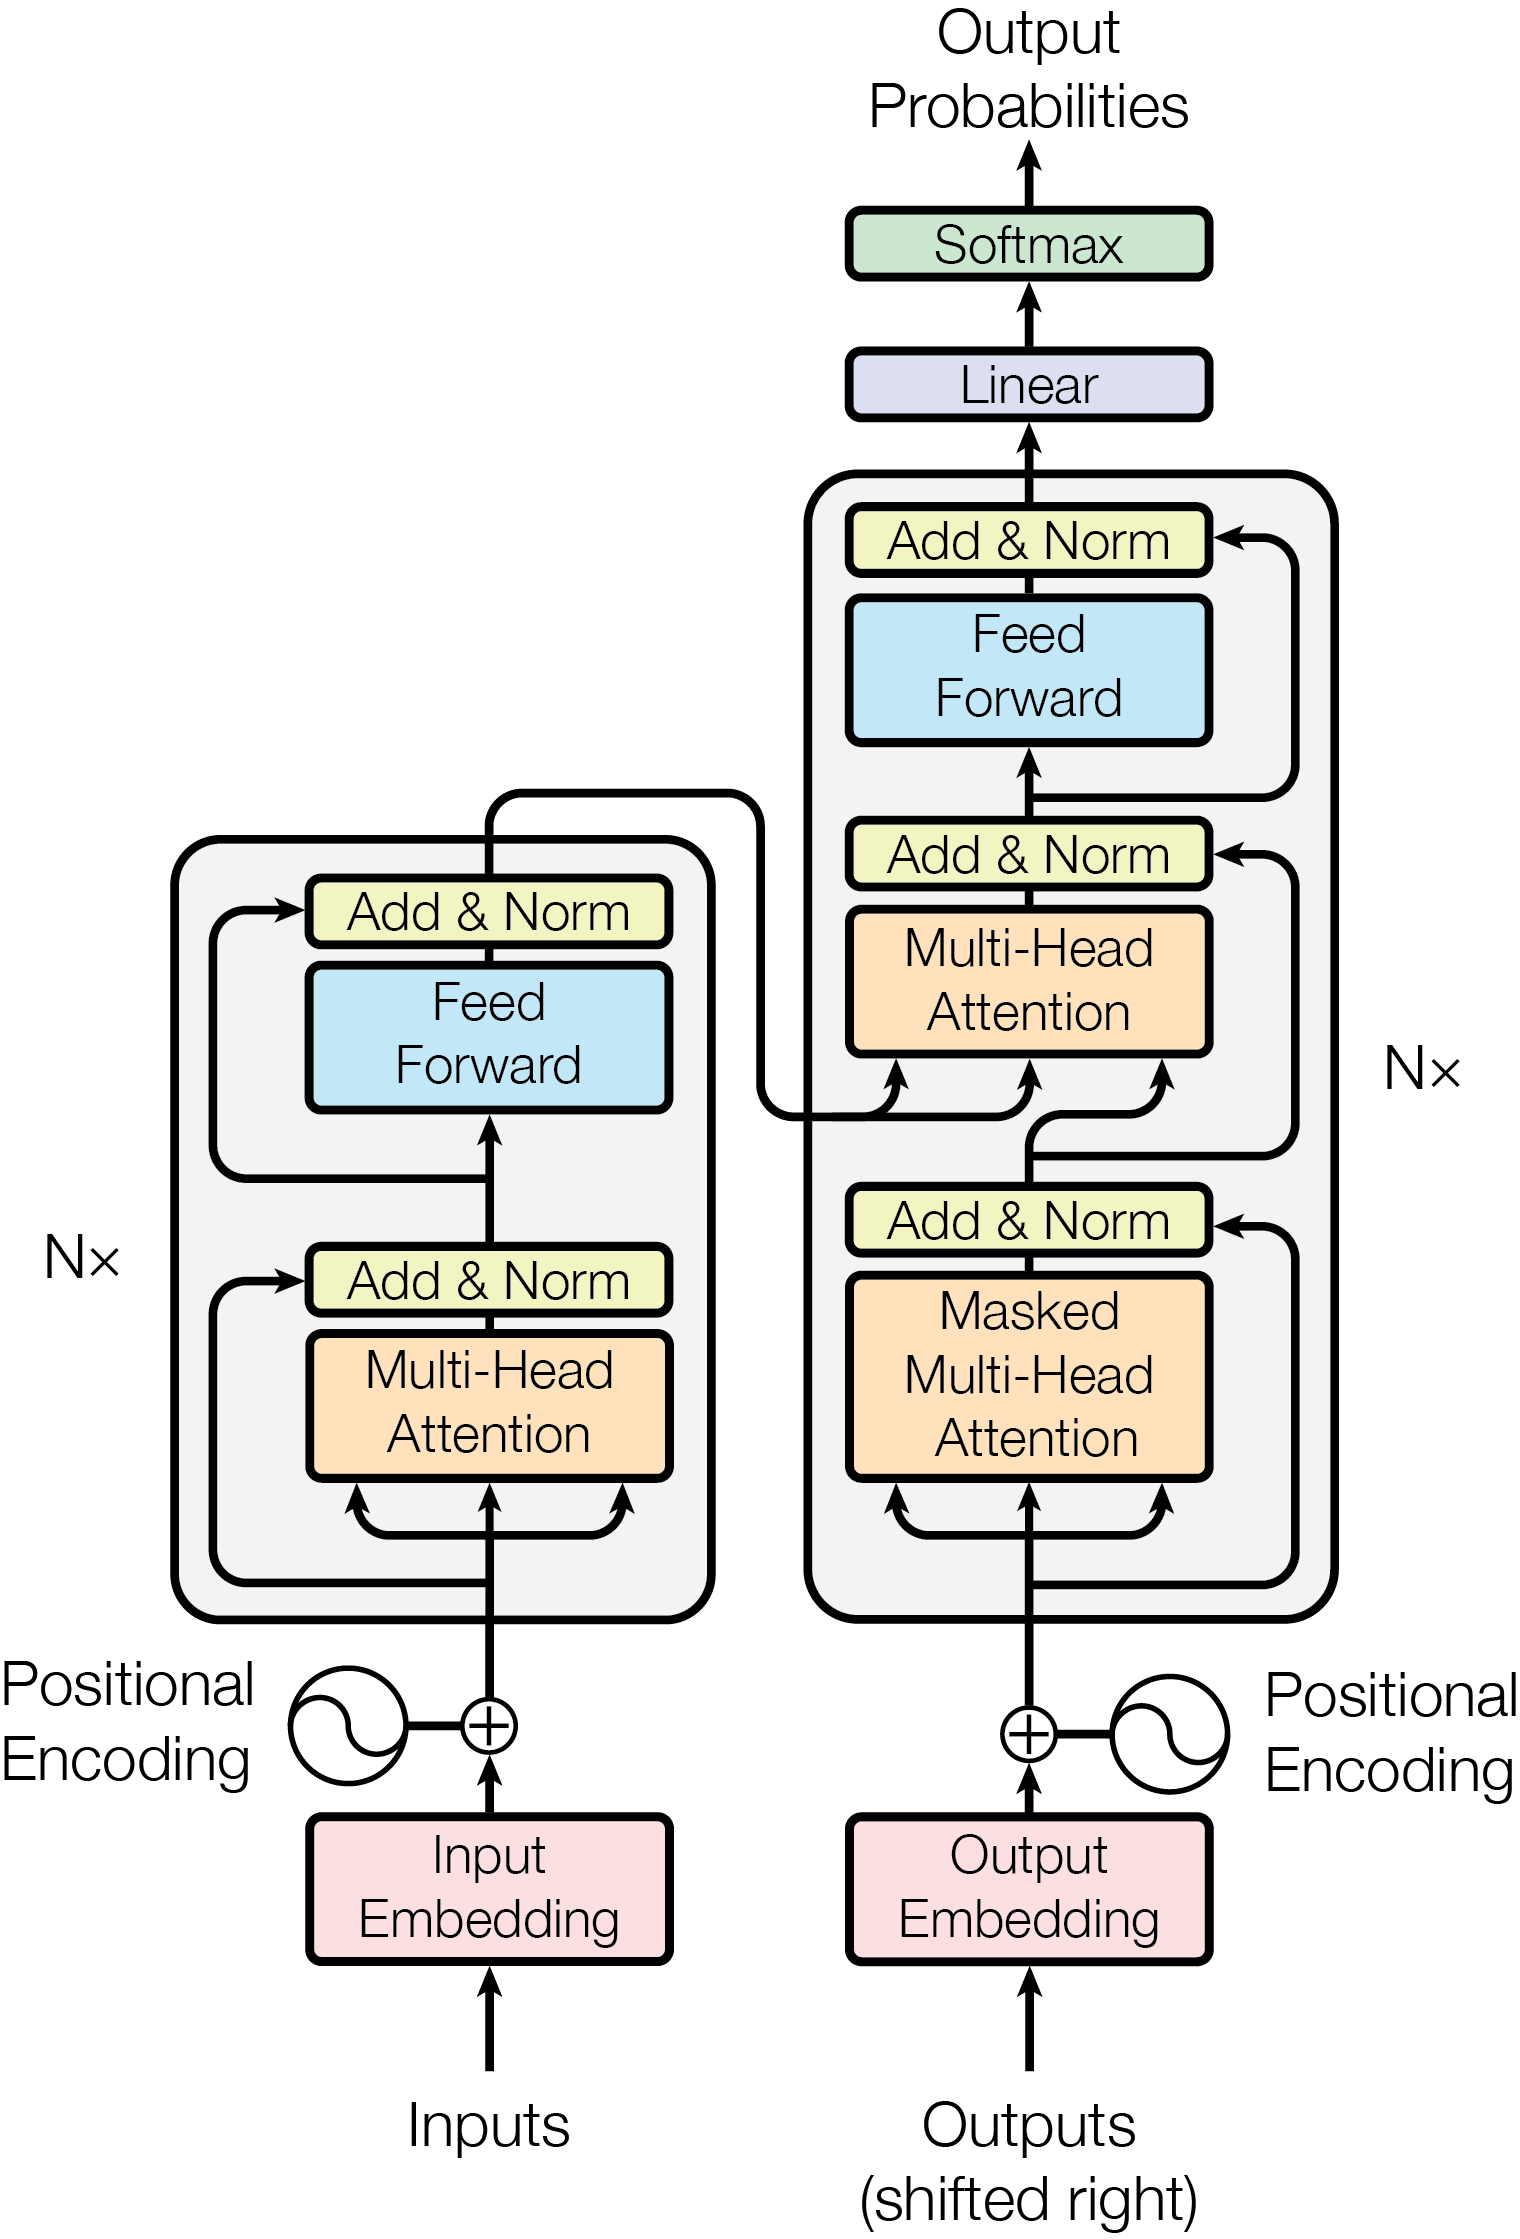
\includegraphics[scale=0.15]{Images & Logos/Transformers.png} 
	\caption{Arquitectura de los Transformers}
	\label{figure:transformers}
\end{figure}
 

Gracias a la capacidad de paralelizacion y de conservar la relación entre palabras distantes del texto que presentan los Transformers, es posible entrenar un modelo de lenguaje con grandes volúmenes de informacion para de esta manera, contar con una red con un gran poder predictivo. Es así como\cite{devlin2018bert}  desarrolla un modelo basado en Transformers capaz de aprender el contexto del lenguaje de una manera general y luego utilizar lo aprendido para distintas tareas de NLP denominado BERT (Bidirectional Transformers for Language Understanding). Para ello se utilizo una arquitectura en donde las capas de entrada son las representaciones vectoriales de las palabras (Embedings) y a partir de ahí, contiene múltiples capas de Transformers. Para su entrenamiento, se suministran dos oraciones consecutivas con palabras faltantes y se asignan dos tareas simultaneas: saber que palabra podría ser la faltante, ademas de identificar el orden de las oraciones. Esto le permite al modelo aprender del contexto del lenguaje a nivel de palabras usando las que vienen antes y después como fuente de información, así como del contexto de las oraciones al identificar su orden. Para ello se utilizo toda la wikipedia. Este modelo pre entrenado es luego capaz de utilizar esta representación contextual del lenguaje para realizar distintas tareas de NLP tales como análisis de sentimiento, al agregar una capa final a la red que produzca un posible resultado, una funcion softmax por ejemplo que permite asignar la probabilidad de pertenencia a algunas de las clases y comparar este resultado con su respectivo valor esperado. El esquema de esta arquitectura se puede apreciar en \ref{figure:BERT} \cite{devlin2018bert}.

\begin{figure}[t]
	\centering
	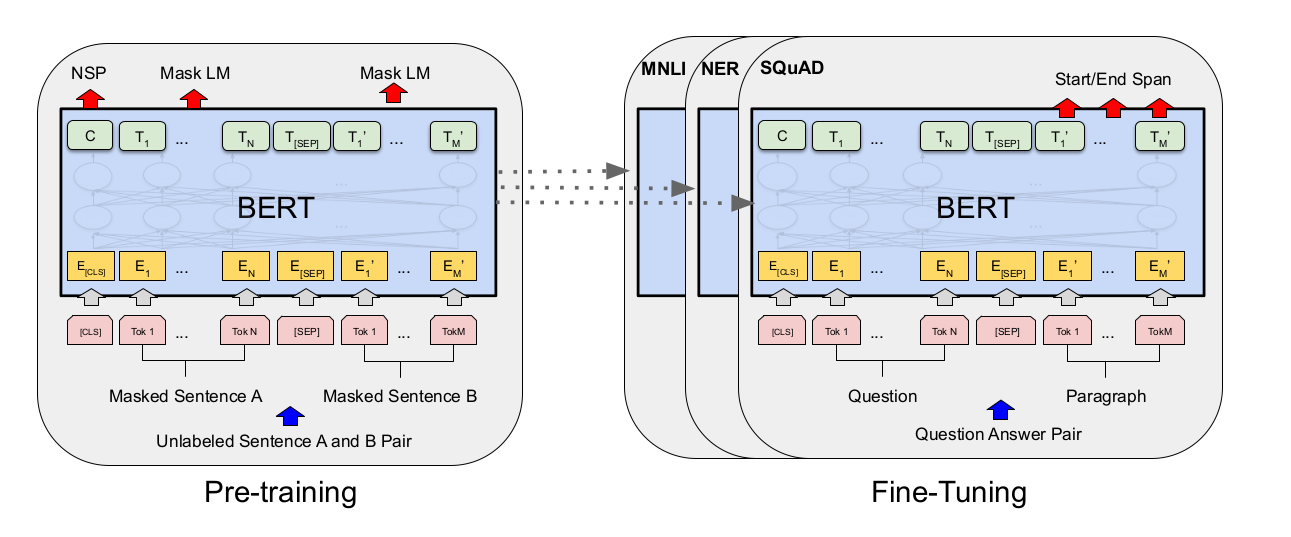
\includegraphics[scale=0.35]{Images & Logos/BERT.png} 
	\caption{Arquitectura de BERT}
	\label{figure:BERT}
\end{figure}



En cuanto a la aplicación de modelos tipo BERT en español, en \cite{canete2020spanish}, los autores resaltan que no existía hasta la fecha un modelo de este tipo entrenado específicamente para este lenguaje, ademas del BERT para múltiples lenguajes. Por ello, se proponen entrenar dicho modelo usando ademas de la Wikipedia en español, texto de publicaciones de las naciones unidas, gobiernos y charlas TED. El resultado fue un modelo que supera al BERT en múltiples idiomas para el español en casi todas las tareas evaluadas.



\section{Sentimientos y emociones en redes sociales}

El campo de estudio de análisis de sentimiento del texto en Internet, ha venido ganando importancia tal como lo describe \cite{pang2008opinion} , tanto para usuarios individuales como para la industria de la publicidad, el mercado financiero y la academia, por lo que se hace un recuento de las distintas técnicas y aplicaciones que son consideradas relevantes por los autores hasta la fecha.

Un espacio particular en donde los usuarios individuales pueden generar grandes volúmenes de informacion sobre distintos contenidos, y por consiguiente, una fuente rica de datos para el análisis de sentimiento son los blogs. Por esta razón, \cite{aman2007identifying} utiliza texto proveniente de ellos para realizar detección de emociones presentes en las oraciones de los mismos. Para este propósito recurren primero a una anotación manual de las mismas y luego a la construcción de features para entrenar distintos modelos supervisados. 

Twitter, un sitio de blogs en particular cuyo formato es el microblogging, es decir, publicaciones pequeñas que se denominan tweets, ha cobrado una gran relevancia en el estudio del texto debido a su gran popularidad entre los usuarios de Internet de todo tipo, desde marcas hasta usuarios individuales y políticos, para abarcar cualquier tema. En ese contexto,  \cite{pak2010twitter} extrae tweets de diferentes usuarios sobre distintos temas para realizar un análisis de sentimientos sobre estos. Para ello se procede  a la identificación de tweets que contengan emoticones felices y tristes, los cuales etiqueta como reflejando un sentimiento positivo o negativo respectivamente, así como tweets provenientes de cuentas de medios de noticias los cuales etiqueta como neutrales. luego se procede a la construcción de features usando n-gramas, a partir de las palabras presentes en el tweets  con los que se entrenan varios clasificadores. 


En \cite{roberts2012empatweet} se identifica la necesidad de contar con un corpus etiquetado que sirva de base para la tarea de identificación de emociones en twitter. Para ello, se seleccionan  14 temas que para los autores tienen un fuerte contenido emocional y las palabras clave asociados a estos para ser usados como hashtags en las extracción. A partir de ahí, manualmente se etiquetaron los tweets con su respectiva emoción. Esto sirvió de base para entrenar un modelo de aprendizaje supervisado y así verificar el poder predictivo de los modelos partiendo de datos etiquetados.


La identificación del sentimiento presente en Twitter puede servir como fuente de aproximación a la realidad social en la que los usuarios se desenvuelven. Por esto,\cite{o2010tweets} se plantea la pregunta si existe una correlación entre el sentimiento encontrado en twitter y las encuestas de opinión. Para ello, se toma una muestra de mil millones de tweets entre 2008 y 2009 y se toman aquellos tweets que contengan palabras claves asociadas a los temas que se están investigando. EL sentimiento de estos tweets se determina a partir de la proporción de palabras con asociación negativa o positiva presentes en el tema que se esta analizando en un día en particular. Los resultados dan una correlación alta entre el sentimiento encontrado a través del texto y las encuestas. Esta relación entre la realidad social y el sentimiento presente en los tweets es también abordada por \cite{bollen2011modeling}, donde se procede a realizar una medida del estado emocional de una muestra de tweets entre agosto y diciembre del 2008, en donde el mismo se mide a través de la similaridad presente entre las palabras de los tweets y ciertos términos claves asociados a estados emocionales. Esto permite encontrar que determinados eventos relevantes generan un impacto emocional significativo y durante un periodo de tiempo considerable en los usuarios.




Al ser el escenario político un caso particular de los fenómenos sociales, cuyo impacto se traduce en el estado emocional de las personas, el sentimiento presente en tweets de contenido político puede dar un indicio de la percepción publica de dicho escenario. Con esto en mente, \cite{tumasjan2010predicting} se plante el uso de twitter como plataforma de medición de la percepción publica respeto a la política durante las elecciones parlamentarias en Alemania en el 2009. Una de sus preguntas de investigación estuvo relacionada con los sentimientos que se reflejan en los tweets que mencionan a los políticos que hacen parte de las campañas, y para esto, usando el texto proveniente de twitter, se utilizo un software capaz de identificar palabras claves asociadas a estados emocionales y cognitivos en el texto. El resultado fue un perfil emocional para cada político que en lineas generales, parece estar de acuerdo con su discurso político.

En \cite{mohammad2015sentiment} se utilizan las elecciones presidenciales de 2012 en estados unidos para elaborar un corpus emocional a partir de tweets relacionados a este tema y etiquetados manualmente con 19 emociones, que luego son agrupadas en 8. Estas tweets sirven para entrenar un modelo de aprendizaje supervisado, siendo de esta manera el trabajo mas cercano y una referencia importante para el presente trabajo.














